\chapter{Results} \label{chap:experiments}

This Chapter describes the experiments done in this work and the results achieved.

\section{Datasets}
Two datasets were used in the experiments, our collected dataset HuPBA-AgeGuess and the classic benchmark database FG-NET.

\textbf{FG-NET} consists of 1002 frontal face images of 82 different individuals. The image quality varies a lot in the dataset since there are images in grey scale and RGB. The face position is frontal and under similar illumination conditions. The dataset also contain 68 facial landmarks for each face image.

\begin{figure}[!h]
	\centering
	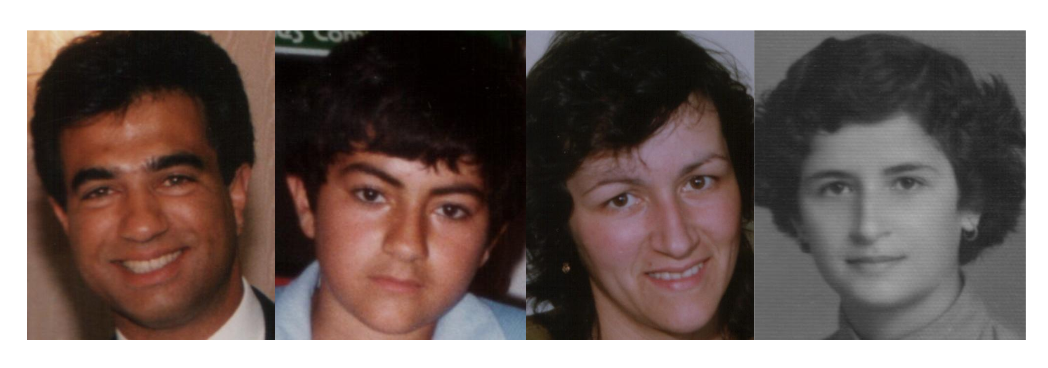
\includegraphics[width=\textwidth]{figures/FGNET_sample}
	\caption{FG-NET image samples.}
	\label{fig:imgSample1}
\end{figure}

\textbf{HuPBA-AgeGuess} dataset (\ref{fig:imgSample2}) used in this project is a subset of the 4865 images filtered out by a minimum number of votes per image. This subset contains 3398 face images. The images are captured in the wild so the faces position vary up to $\pm90º$ and the illumination is also different in every picture.

\begin{figure}[!h]
	\centering
	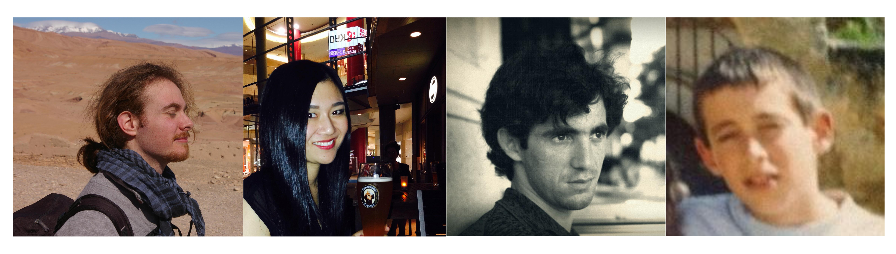
\includegraphics[width=\textwidth]{figures/HuPBA_sample}
	\caption{HuPBA-AgeGuess image samples.}
	\label{fig:imgSample2}
\end{figure}

Given the characteristics of the used descriptors in this work, both databases could be incremented by computing the mirror image, doubling the number of faces of each dataset (i.e. 2004 faces for the FG-NET and 6796 face images for the HuPBA-AgeGuess dataset).

\section{Evaluation Metrics} 

The two most commonly used evaluation metrics in age estimation are \acrfull{mae} and \gls{cs}.

The \gls{mae} is described as,

\begin{equation}
MAE = \frac{1}{n_{s}}\sum_{i=0}^{n_{s}-1} |e_i|,
\end{equation}

where $n_s$ is the number of samples and $e_i$ is the error of the $ith$ instance, i.e. $e_i = |\hat{y_i} - y_i|$ where $y_i $ is the real label and $\hat{y_i}$ is the predicted label. This metric tells the average number of years that the prediction is wrong.

\gls{cs} is defined as the percentage of test images such that the absolute error is not higher than a threshold, $t$ (in years). i.e.,

\begin{equation}
CS(t) = (1 - \frac{1}{n_{s}}\sum_{i=0}^{n_{s}-1} h(|\hat{y_i} - y_i| - t))\cdot 100
\end{equation}
\begin{equation}
h(x) = 
\begin{cases}
1,				& \text{if } x \geq 0\\
0,              & \text{otherwise},
\end{cases}
\end{equation}

where $y_i$ is the age label of the $ith$ test image and $\hat{y_i}$ is the age prediction of the $ith$ test image.

To evaluate the performance of the age group classifier the accuracy measure is used, modifying the distance measure 

To evaluate the performance of the age group classifier it is needed to take into account that the labels are a disjoint segmentation of the spectrum of possible ages. Therefore, the accuracy measure is used, normalizing the euclidean distance by the number of classes,

\begin{equation}
\text{accuracy} = \frac{1}{n_s}\sum_{i=0}^{n_s-1} \bigg{(} 1-\frac{|\hat{y_i}-y_i|}{n_c}\bigg{)}
\end{equation}

where $n_c$ is the number of different classes. This measure qualifies the predictions based on how close they are from the real label. 

\section{Experimental Settings}
This section describes the experimental setup and the parameters used in the two proposed methods.

\subsection{Biologically Inspired Method}

As described in Section \ref{sec:BIF} a \gls{svm} classifier and three \gls{svr} regressors were trained for this method. 

In order to find the best parameters a grid search was performed to find the best parameters. The parameters that formed the search space were the ones required by the \gls{svm} and \glspl{svr} and its kernels, which are the following:

\begin{itemize}
	\item \textbf{Penalty term ($C$)}: This is the Support Vector parameter that deals with the cost of a misclassification over all the classification task. 
	
	The $C$ parameters tried in the search space were between 0.1 and 2. The best parameters in the Age Group Classification were between 1 and 2 and the best parameters for the \glspl{svr} were between 0.1 and 1.
	
	\item \textbf{Influence term ($\gamma$)}: It is the \gls{rbf} kernel parameter. It determines how far the influence of a single training example reaches.
	
	The $\gamma$ parameters used were between 0.001 and 1, being between 0.001 and 0.01 the ones with better performance.
\end{itemize}

In order to train and validate the parameters a nested 10-fold cross validation technique was used.

\subsection{Deep Learning Method}

In order to validate and test the method a 10-fold cross validation was performed splitting the data into $80\%$ training set, $10\%$ validation set and $10\%$ testing set. The data was split into batches each of them containing 213 instances. In this way each fold will contain an exact number of batches, 3. The error function used during the training was the mean square error. The network also needs the following parameters to be set,

\begin{itemize}
	\item \textbf{Learning Rate ($\eta $)}: The learning rate is used in the backpropagation stage to modify the net weights.
	
	The learning rate used in the experiments was set to 0.002. 
	
	\item \textbf{Epoch}: In training a neural network, the term epoch is used to describe a complete pass through all of the training patterns. The error is reduced over the epoch since the weights are updated within each epoch.
	
	The number of epochs used in the training of the proposed \gls{cnn} were 400.
\end{itemize}

\section{Analysis of the Experiments}

% además de la discusión de los resultados recuerda poner muchas imágenes:

%-ejemplos de landmark fitting (1 página de imágenes)

%-imagenes ejem de perfecto reconocim- algunas que fallen.

%-en el caso de deep learning estaría bien mostrar las features encontradas!!!!! (los filtros) e incluso el resultado de aplicar los filtros a imagenes de caras !!!!

%incluir discusion de pros contras y comparativa de los 2 métodos.

%cuando lo tratas como multi-clasificación mostrar visualmente con colores la matriz de confusión

In this section the results of all the experiments is described and analysed in detail. The experiments were run in the two datasets, FG-NET and HuPBA-AgeGuess, amd with the two different age labels (just in HuPBA-AgeGuess).

\subsection{Face Detection and Alignment}

This preprocessing step was just applied to the HuPBA-AgeGuess dataset since the FG-NET already contains the 68 facial landmarks manually placed. The database HuPBA-AgeGuess was preprocessed as described in Section \ref{sec:preproces}. The face detection was $92.52\%$ accurate and face alignment was $84.54\%$ accurate, hence the total accuracy of the preprocessing was $78.26\%$. Some examples of good and bad face detections and alignments are shown in Figure \ref{fig:sampPP}.

\begin{figure}[!h]
	\centering
	\begin{subfigure}[b]{\textwidth}
		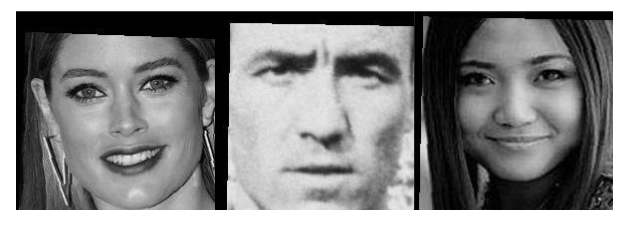
\includegraphics[width=\textwidth]{figures/good_pp}
		\caption{Well detected and aligned faces.}
		\label{fig:goodPP}
	\end{subfigure}%
	
	 %add desired spacing between images, e. g. ~, \quad, \qquad, \hfill etc.
	%(or a blank line to force the subfigure onto a new line)
	\begin{subfigure}[b]{\textwidth}
		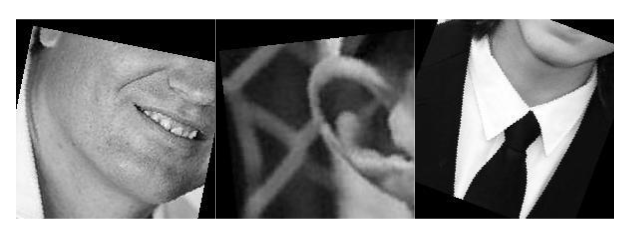
\includegraphics[width=\textwidth]{figures/bad_detection}
		\caption{Samples of bad face detection.}
		\label{fig:badDet}
	\end{subfigure}
	
	 %add desired spacing between images, e. g. ~, \quad, \qquad, \hfill etc.
	%(or a blank line to force the subfigure onto a new line)
	\begin{subfigure}[b]{\textwidth}
		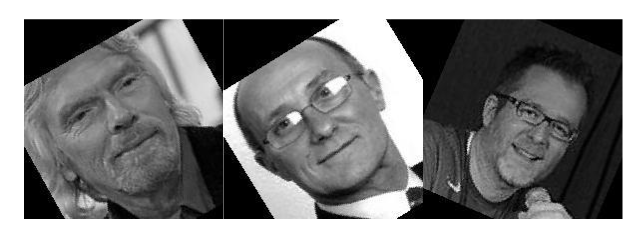
\includegraphics[width=\textwidth]{figures/bad_alignment}
		\caption{Samples of bad face alignment.}
		\label{fig:badAl}
	\end{subfigure}
	\caption{Samples of preprocessed faces.}\label{fig:sampPP}
\end{figure}

The detection and alignment were tricky since the images are not taken in a controlled environment, the multiple illumination changes and the multiple head orientations made the preprocessing very difficult.

\subsection{Biologically Inspired Method}

The \gls{mae} achieved by this method in both databases is shown in the Table \ref{tab:BIFresults}. As it was expected the algorithm performed better with the FG-NET dataset since the landmarks were manually placed. Between both experiments with the HuPBA-AgeGuess dataset this method performed best in the apparent age labels.

\begin{table}[!h]
	\centering
	\begin{tabular}{|l||c|}
		\hline
		\multicolumn{1}{|c||}{\textbf{Database}} & \textbf{\gls{mae}}\\ \hhline{=#=}
		FG-NET & $7.99$\\ 		\hline
		HuPBA-AgeGuess real age & $10.73$\\ \hline
		HuPBA-AgeGuess apparent age & $9.34$\\ \hline
			
	\end{tabular}
	\caption{\gls{mae} achieved with \gls{bif}.}
	\label{tab:BIFresults}
\end{table}

Figure \ref{fig:cumS_BIF} shows the \gls{cs} obtained with this method. It shows that the performance is better over apparent age than real age.

\begin{figure}[!h]
	\centering
	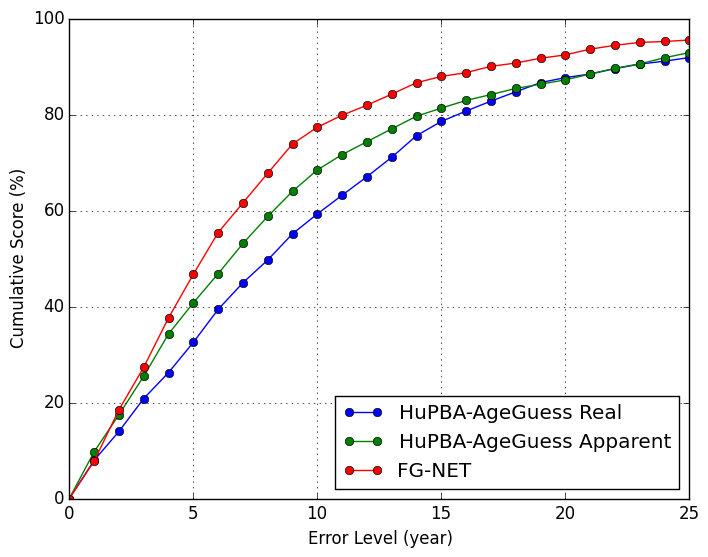
\includegraphics[width=\textwidth]{figures/cum_score}
	\caption{\gls{cs} achieved with the Biologically Inspired Method.}
	\label{fig:cumS_BIF}
\end{figure}

The group classification achieves a $0.895$ accuracy with FG-NET and $0.87$ with HuPBA-AgeGuess dataset. Figure \ref{fig:cm} shows the confusion matrix obtained in each one of the three datasets.

\begin{figure}[!h]
	\centering
	\begin{subfigure}[b]{0.5\textwidth}
		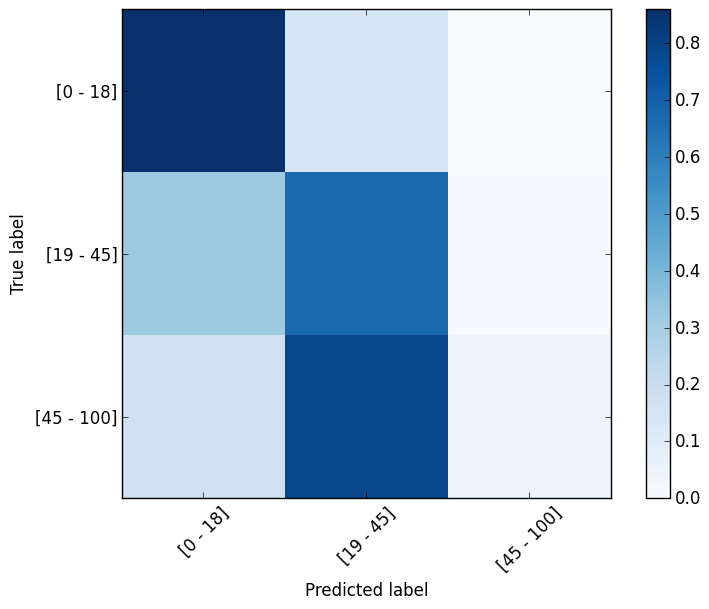
\includegraphics[width=\textwidth]{figures/FG-NETconf_mat}
		\caption{FG-NET dataset.}
		\label{fig:cmfgnet}
	\end{subfigure}%
	~
	%add desired spacing between images, e. g. ~, \quad, \qquad, \hfill etc.
	%(or a blank line to force the subfigure onto a new line)
	\begin{subfigure}[b]{0.5\textwidth}
		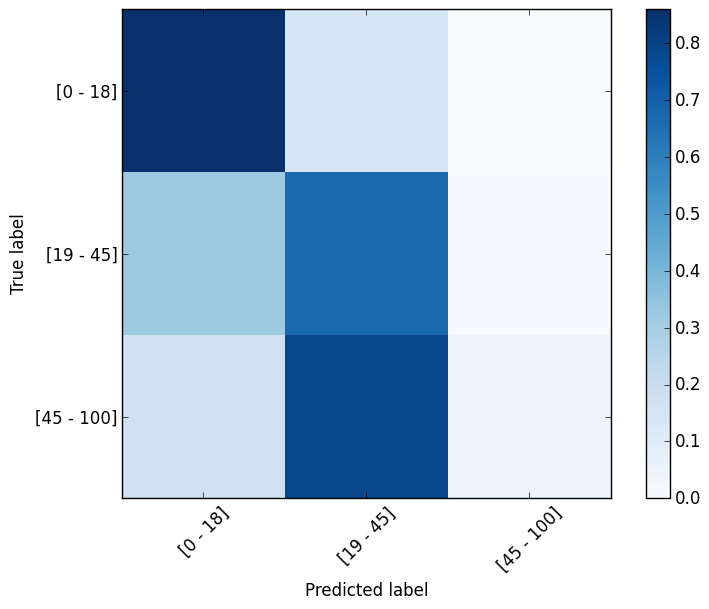
\includegraphics[width=\textwidth]{figures/FG-NETconf_mat}
		\captionsetup{width=1.1\textwidth}
		\caption{HuPBA-AgeGuess with Real Age labels.}
		\label{fig:cmreal}
	\end{subfigure} %
	
	%add desired spacing between images, e. g. ~, \quad, \qquad, \hfill etc.
	%(or a blank line to force the subfigure onto a new line)
	\begin{subfigure}[b]{0.5\textwidth}
		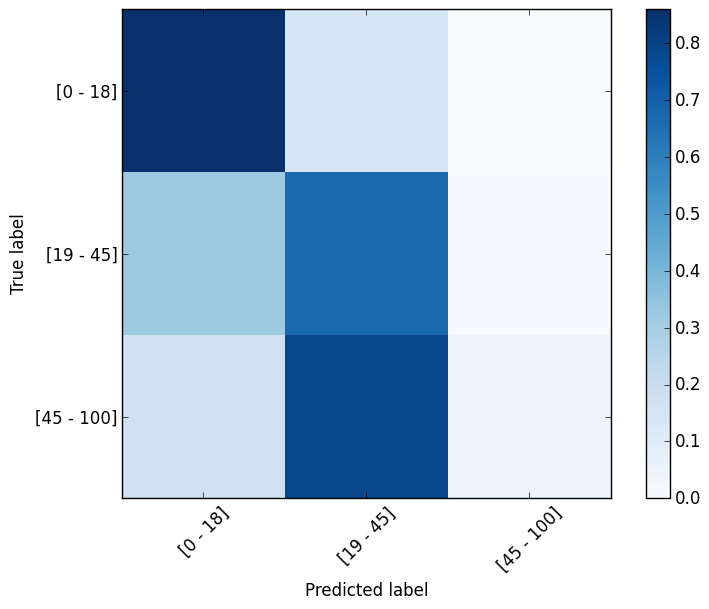
\includegraphics[width=\textwidth]{figures/FG-NETconf_mat}
		\caption{HuPBA-AgeGuess with Apparent Age labels.}
		\label{fig:cmapp}
	\end{subfigure}
	\caption{Confusion Matrices of the Age Group Classification.}\label{fig:cm}
\end{figure}

\note{Study the CS and MAE by group of ages (maybe images in Appendix)}

\subsection{Deep Learning Method}

The Table \ref{tab:CNNresults} shows the achieved \gls{mae} with this method in all three datasets. 

\begin{table}[!h]
	\centering
	\begin{tabular}{|l||c|}
		\hline
		\multicolumn{1}{|c||}{\textbf{Database}} & \textbf{\gls{mae}}\\ \hhline{=#=}
		FG-NET & \\ 		\hline
		HuPBA-AgeGuess real age & $10.29$\\ \hline
		HuPBA-AgeGuess apparent age & $8.71$\\ \hline
		
	\end{tabular}
	\caption{\gls{mae} achieved with \gls{cnn}.}
	\label{tab:CNNresults}
\end{table}

\note{Show weight masks (maybe in the Apendix)}

\subsection{Comparison}


In both methods can be appreciated that the performance is higher with apparent age estimation than real age estimation. 

In both \gls{cnn} and \gls{bif} methods the FG-NET dataset achieved better results. This is because the images in that dataset are frontal faces and the 68 landmarks were manually placed, while the HuPBA-AgeGuess database contains non frontal face images and the landmarks are automatically regressed.

\begin{table}[!h]
	\centering
	\begin{tabular}{|l|l|c|}
		\hline
		\multicolumn{1}{|c|}{\textbf{Method}} & 
		\multicolumn{1}{|c|}{\textbf{Database}} & \textbf{\gls{mae}}\\ \hline\hline%\hhline{====}
		\multirow{3}{*}{Bio-Inspired Method} & FG-NET & $7.99$\\ 		\cline{2-3} 
		& HuPBA-AgeGuess real age & $10.73$\\ \cline{2-3}
		& HuPBA-AgeGuess apparent age & $9.34$\\ \hline\hline%\hhline{====}
		\multirow{3}{*}{CNN Method} & FG-NET & \\ \cline{2-3}
		& HuPBA-AgeGuess real age & $10.29$\\ \cline{2-3}
		
		& HuPBA-AgeGuess apparent age & $8.71$ \\ \hline
		
		
	\end{tabular}
	\caption{\gls{mae} of the different experiments.}
	\label{tab:results}
\end{table}